\section{Low Level Motion}
In low level motion planning layer of the agent architecture we needed a robust algorithm capable of compensating possible noise incurred by output of vision stack.  The simple goal for this part is to make robot capable of following a path to reach a destination position determined by higher levels of path planning algorithm.
\subsection{Potential Field}
To achieve the goal stated above we started with implementing Potential Fields\cite{paper:PF} algorithm. This algorithm is a well-known method for robot path planning. It has several properties which makes it suitable for our application. The behaviour of the algorithm is completely reactive and therefore if it is fed with noisy input in one cycle it will be able to recover in next cycles, therefore performance of the algorithm degrades as amount of noise increases never failing completely.
\subsection{Challenges}
During implementation of this method, we had several challenges. We started testing this algorithm for milestone two but failed. The initial intuition for most members was that the failure was due to complexity of this algorithm while the failure was in fact due to unreliable input produced by vision stack. Later, new set of tests showed a very good performance once the vision stack become robust and reliable. Successful implementation of this algorithm was a key to our success in third and fourth friendly matches.
\subsection{Kinematic Model and Implementation}
In order to implement this algorithm successfully we needed to find a way to apply the calculated velocity vector from previous step on the robot. To do this, we used a kinematic model of a differential drive robot. In figure \ref{KinModel},the velocity vector is decomposed into linear and angular velocity and later they are fused to calculate velocity of left and right wheels.
\begin{figure}[htp]
\begin{center}
\leavevmode
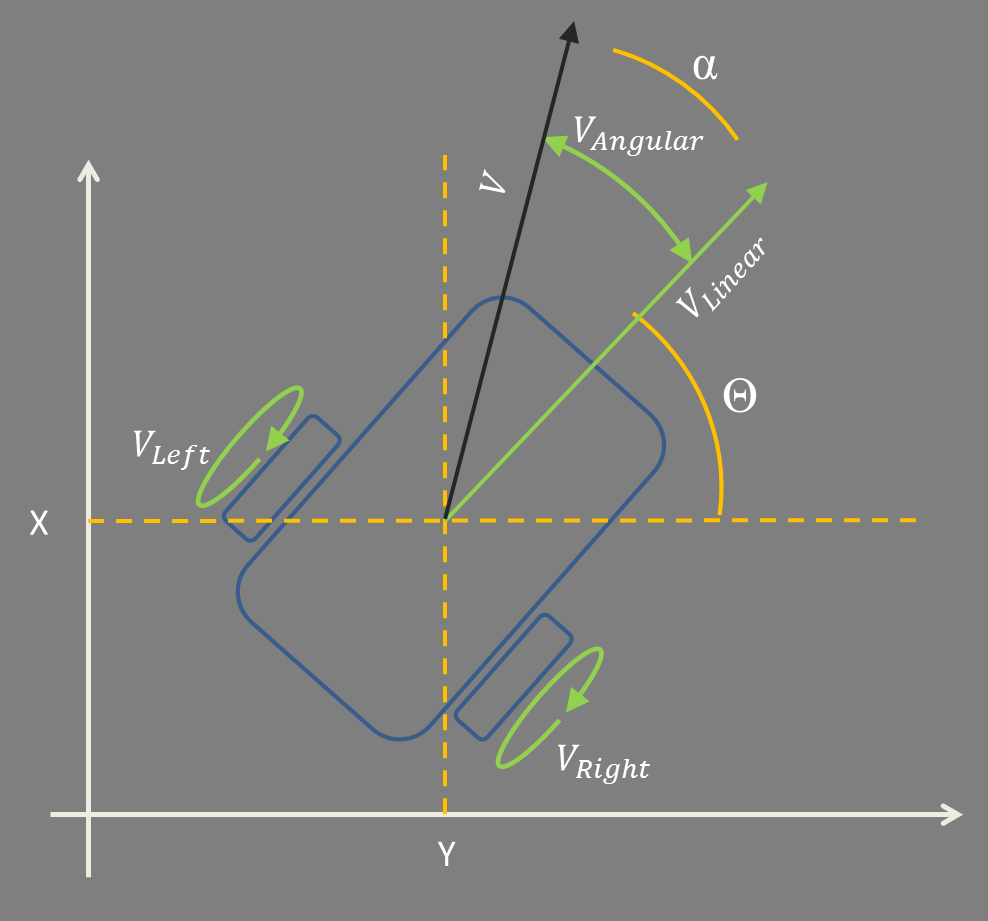
\includegraphics[width=0.25\textwidth] {KinModel.png}
\end{center}
\caption{Kinematic Model of Non-holonomic Differential Drive Robot}
\label{fig:KinModel}
\end{figure}
\begin{align}
V & =k_{att}.(Pos_{current}-Pos_{destination})\\
V_{linear} &= \begin{Vmatrix}v\end{Vmatrix} cos(\theta) ,
V_{angular} = {K\theta \over \pi}\\
V_{left}&=V_{Linear}-rsin(V_{Angular})\\
V_{right}&=V_{Linear}+rsin(V_{Angular})
\end{align}

Integrating all this we were able to implement a successful motion planning algorithm which distinguished our team from other teams.
\subsection{Results and Lessons Learned}
A sample result of running this algorithm on the pitch is demonstrated in figure \ref{fig:seq}, Overall, this algorithm could deal with almost all scenarios successfully and when integrated with a high level decision making layer, we had a reliable game play scenario. 
The solution also can also deal effectively with obstacles using Extended Potential Field algorithm\cite{paper:OKhatib} but this feature was not used because obstacle avoidance was dealt with by higher levels of decision making. Therefore, the algorithm at this level is a conventional P controller.  

\begin{figure}[htp]
\begin{center}
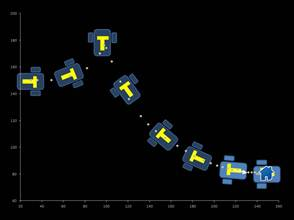
\includegraphics[width=0.25\textwidth] {Final.jpg}
\caption{Complete Robot movements from start position to destination position.}
\label{fig:seq}
\end{center}
\end{figure}
\subsection{Lessons Learned}

\begin{itemize}
\item It is possible to implement reliable applications based on ideas developed in research labs. 
\item Failure of an algorithm at higher levels sometimes may be due to invalid inputs from lower layers.
\item Simulation at abstract level is very useful for making sure that an algorithm is developed according to specification but successful implementation based on such simulation environments does does not guarantee optimal performance in real environments.
\end{itemize}